\documentclass{article}
\usepackage[utf8]{inputenc}
\usepackage{amssymb}
\usepackage{tikz}
\usepackage{amsmath}
\usepackage{relsize}
\usepackage{mathtools}
\usepackage{textcomp}
\usepackage{eurosym}
\usepackage{graphicx}
\usepackage[autopunct=true]{csquotes}

\title{Labbook \\ Learning in Social Networks}
\author{Roman Oort 12189030\\ r.s.oort@gmail.com\\[1cm]{\normal Supervisor: Adrian Haret}}
\date{\today}
\DeclareMathOperator*{\plim}{plim}
\begin{document}

\maketitle
\newpage
\section{First Week}
\subsection{8/4/2021}
Started implementing network generation. Generated networks need to be aperiodic, stochastic and positive.

The code is contained in the Network class, at the moment containing the code for generating a network, adhering the to previously mentioned constraints, and the ability to grow that network. Furthermore a basic function was added to verify the generated networks do indeed converge. 

To grow the network an incremental approach was used, to ensure that the networks would satisfy the constraints at every time step. This worked by generating a square, zero, array which was a single agent larger than the previous array. The contents of the old array were then copied into this new array to maintain the same structure between iterations of the network.\newline
This method was indeed successful in creating networks that satisfy the aforementioned conditions.

However, this method was replaced in favour of a slightly different, though still incremental, updating procedure. Instead of generating an entirely new array at every time step the function was adjusted to expand the already existing network by concatenating a new row and column the already existing array. This adjustment lead to an $\sim 10 \times$ speed up in the generation time.

To ensure that the generated networks are strongly connected at every time step as each agent $i$ gets added they are guaranteed to receive both an incoming and outgoing link as they are added to the network. The receiving and sending agents for these links are chosen randomly, from an uniform distribution from the agents already present in the network.

As a side-effect this gives a natural bias towards the older agents in the network, w.r.t. degree distribution. Those agents that are present longer in a society will tend to have more connections than newcomers.

As this is just the basis for the network all weights in the network are equal.

To ensure the network is aperiodic the first agent in the network is guaranteed to get a self-link, meaning a weight to itself. For all other agents the chance whether they have a self-link is determined by an optional parameter, which defaults to 1, making it so that every agent has a self-link.

\newpage

\subsection*{10/4/2021}
A function was implemented to generate the truth value of the world, and the signals sent to the agents.
The truth of the world, $mu$, is drawn from a uniform distribution over the interval $[0, 1]$. At $t=0$ each agent receives a noisy signal, $\mu + \epsilon_i$, of this true world state, where $\epsilon_i$ is a zero-mean normally distributed variable, with $\sigma^2 = \mu^2$. As each agent gets added to the network it also adds a new noisy signal to the belief vector $\textbf{p}$.

The generation method was also altered to increase the generation speed. Instead of an incremental approach the network is created at a pre-determined size, without any weight. By iterating over the agents each agents gets their respective links added, one incoming and one outgoing, from the already present agents in the network, to ensure fully connectedness at every $t$. To use the smaller networks in the computation of the convergence one can simply take a slice of the array of the desired size.

This managed to decrease the generation time from, seemingly, polynomial to linear time, greatly decreasing the network generation time, as can be seen in figure \ref{time:2} below.
\begin{center}
    \begin{figure}[!htbp]
        \centering
        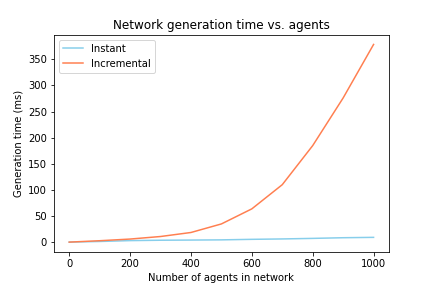
\includegraphics[width=1\textwidth]{GenTime2.png}
        \caption{Network Generation Time, Mean over 10 Iterations}
        \label{time:2}
    \end{figure}
\end{center}
\newpage
Additionally a method to increase the degree distribution in the network has been implemented. This uses an additional, optional, flag as parameter to use this function. When this flag is set to true, when generating the links for the network, each agent is assigned an additional, ranndom, number of incoming and outgoing links. These numbers are drawn randomly, from a 2 mean normal distribution, with $\sigma^2=1$, which are then rounded to integers. Then for the determined number of additional links the other agents involved in the link are drawn randomly, from a uniform distribution over the agents in the \emph{entire} network. This increases the degree distribution off the overall network and slightly decreases the bias on the earlier agents in the network, while not removing it entirely. The results can be seen in figure \ref{degree:increase} below.
\begin{center}
    \begin{figure}[!htbp]
        \centering
        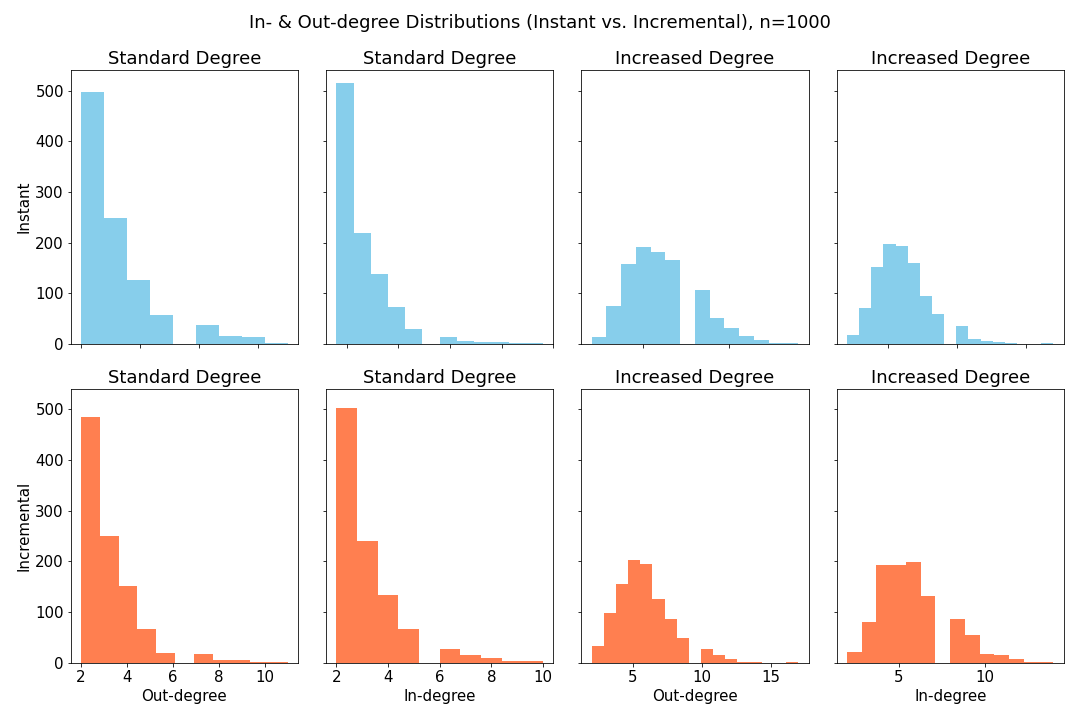
\includegraphics[width=1\textwidth]{ThesisKI/IncrementalVSInstantDegree.png}
        \caption{Degree Distribution Comparison}
        \label{degree:increase}
    \end{figure}
\end{center}
\end{document}
